\chapter{Az S-gráf keretrendszer}
Az S-gráf keretrendszer volt az első publikált gráf elméleten alapuló módszer szakaszos gyártórendszerek ütemezési problémáinak megoldására. \cite{Sanmarti2002}
A keretrendszer egy irányított gráf modellből, az S-gráfból és a hozzá tartozó algoritmusokból áll. \cite{SANMARTI1998S847}
Az S-gráf egy speciális irányított gráf, amely nem csupán a probléma vizualizációjára képes, hanem egy matematikai modell is.
A keretrendszerben a recepteket, valamint a félkész-, illetve a teljes ütemterveket is az S-gráf reprezentálja.
Ezekben a gráfokban a termékeket, illetve a feladatokat a pontok jelölik, amelyeket csomópontoknak nevezünk.
Ezenkívül, ha két feladat között összeköttetés van, ezt a gráfon a két feladatot reprezentáló csomópontok közötti nyíl jelöli.
Az ütemezési információ nélküli S-gráfot recept gráfnak (\textbf{recipe graph)} nevezzük, melyre egy példa a \ref{recipeGraph} ábrán látható.
\begin{figure}[H]
\begin{center}
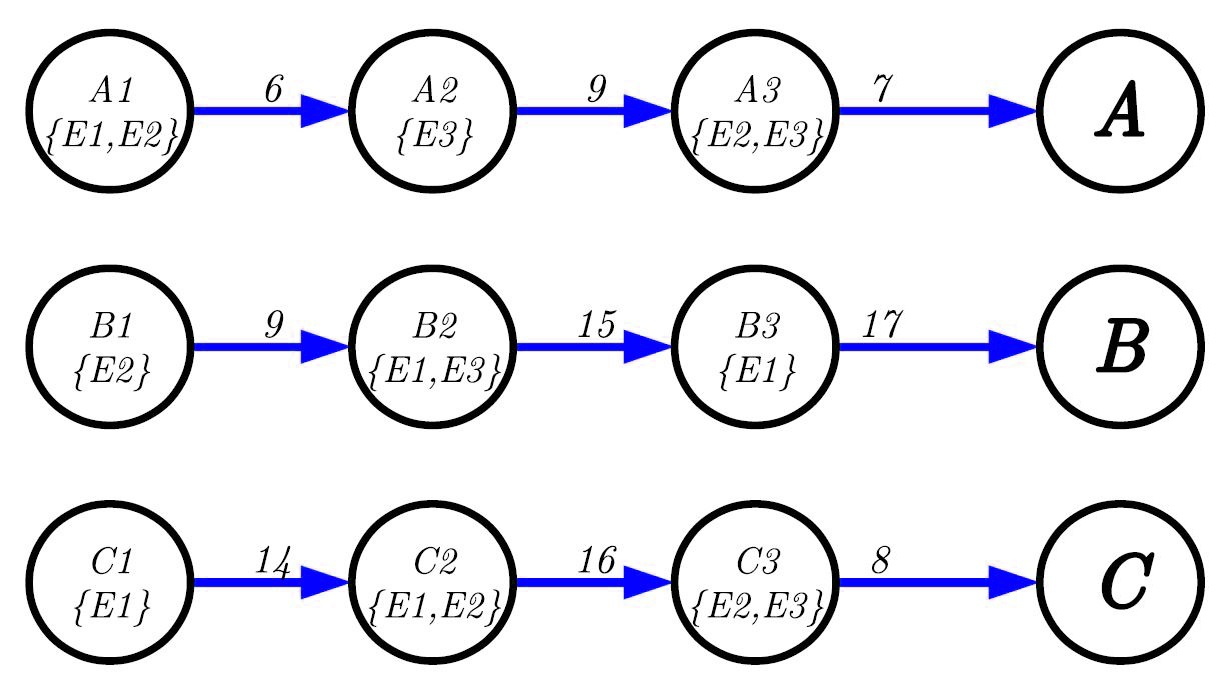
\includegraphics[scale=0.35]{recipeGraph}
\caption{A recept gráf szemléltetése}
\label{recipeGraph}
\end{center}
\end{figure}
Az ábrán látható jobb oldali három csomópont (A,B,C) jelöli a termékeket, a többi csomópont pedig a részfeladatokat, amelyeket el kell végezni a termékek előállítása érdekében.
A recept gráf nyilai reprezentálják egyrészt két részfeladat közötti függőséget, abban ez esetben például, ha ez egyik részfeladat állítja elő a másik részfeladathoz szükséges bemeneti részterméket, másrészt a részfeladatok és a késztermékek közötti függőséget.
A recept gráf minden részfeladathoz tartozó csomópontjához tartozik egy halmaz, amely azon berendezések nevét tartalmazza, amelyek képesek adott részfeladat megoldására.
A nyilakon található súlyok pedig a részfeladat megoldásához szükséges gyártási időt reprezentálják, abban az esetben, ha egy részfeladatot több berendezés is el tud végezni, a nyíl súlya a berendezésekhez tartozó gyártási idők közül a legkisebb lesz.

Az S-gráf keretrendszerben található algoritmusok az előzőekben bemutatott recept gráfot egészítik ki ütemezési nyilakkal, amelyek az algoritmus által meghozott ütemezési döntéseket reprezentálják.
Az ily módon előállított gráfot, függetlenül attól, hogy van-e még meghozatlan ütemezési döntés, vagy pedig a teljes ütemezés megtörtént, ütemezési gráfnak (\textbf{schedule graph}) nevezzük.
A \ref{recipeGraph} pontban látható recept gráf alapján előállított ütemezési gráf a \ref{scheduleGraph} ábrán látható.
\begin{figure}[H]
\begin{center}
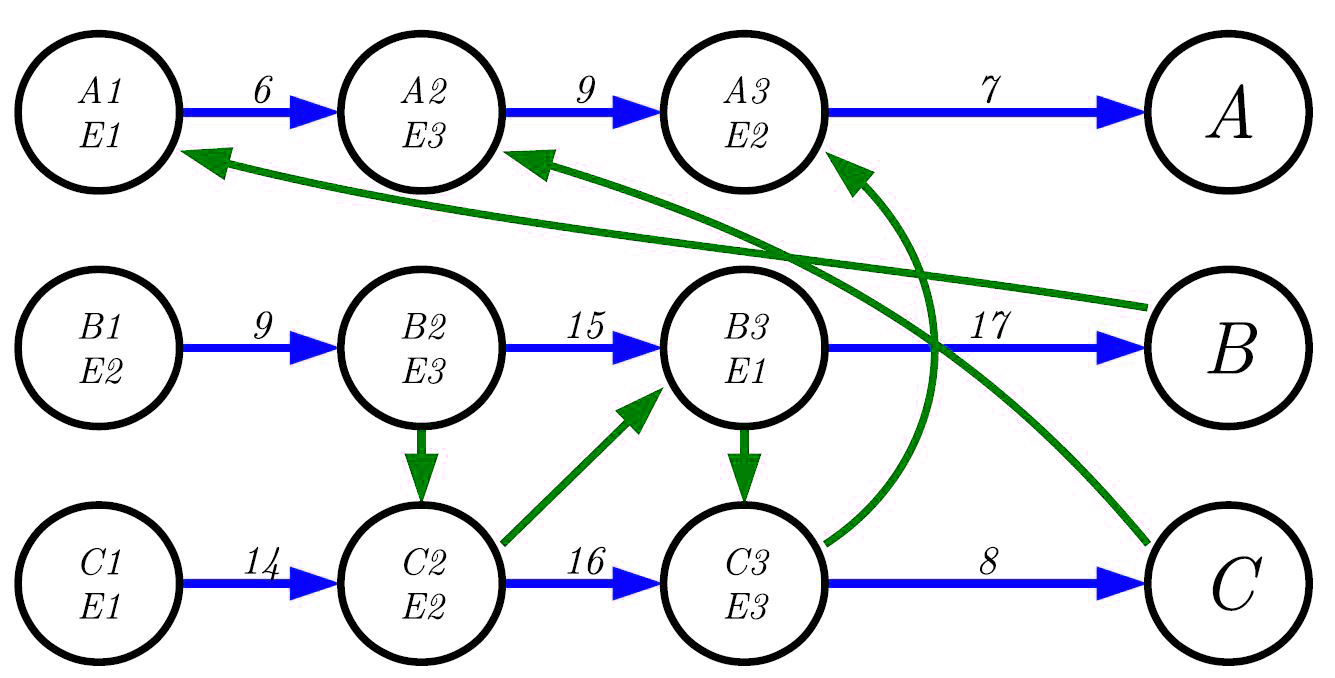
\includegraphics[scale=0.3]{scheduleGraph}
\caption{Az ütemezési gráf szemléltetése}
\label{scheduleGraph}
\end{center}
\end{figure}
Az ábrán látható gráfon már minden ütemezési döntés lezajlott, a zöld nyilak jelölik az ütemező algoritmus által behúzott ütemezési nyilakat.
A részfeladatokat reprezentáló csomópontokon immáron a lehetséges berendezések halmaza helyett egy konkrét berendezés jelölése található, amely az adott részfeladat elvégzésére hivatott az adott ütemterv szerint.
Az ütemezési nyilak súlya alapértelmezetten $0$, ha az adott problémában nem számolunk például részfeladatok közötti szállítási-, átállási-, illetve tisztítási időkkel.
Az adott berendezéshez rendelt részfeladatok sorrendje könnyen leolvasható az ütemezési gráfról, erre egy példa a \ref{unitSequence} ábrán látható.
\begin{figure}[H]
\begin{center}
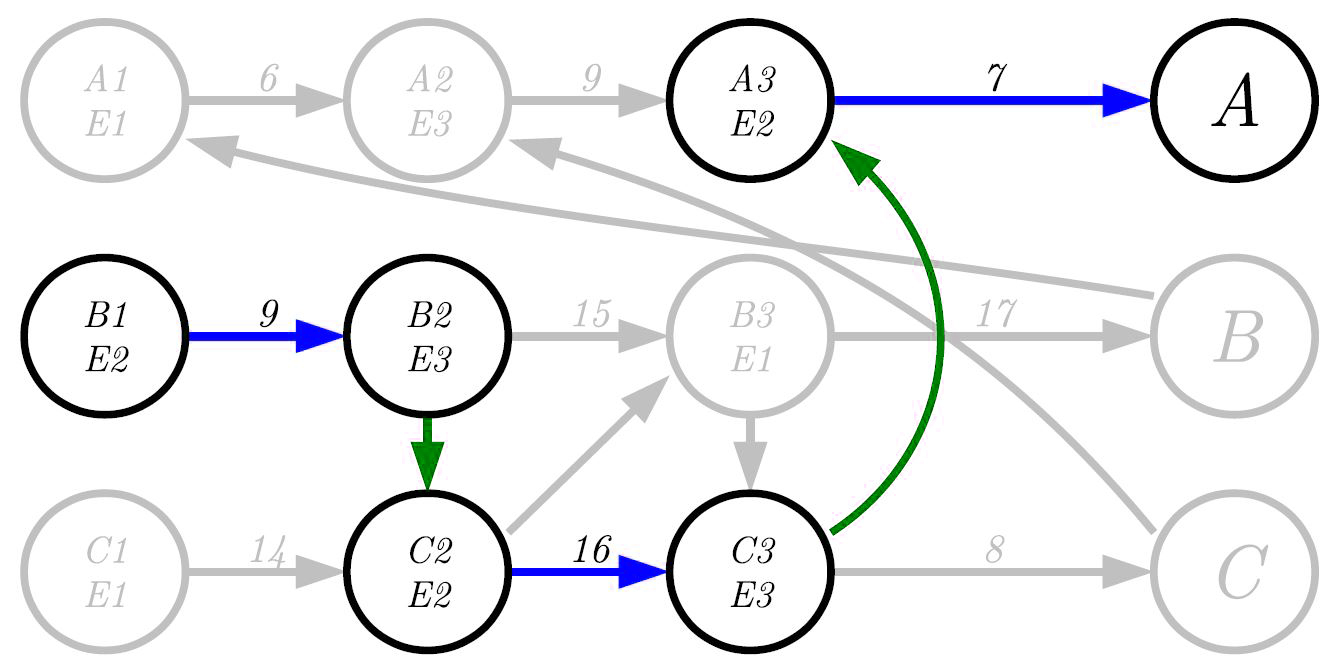
\includegraphics[scale=0.3]{unitSequence}
\caption{Az E2 berendezéshez rendelt részfeladatok sorrendje}
\label{unitSequence}
\end{center}
\end{figure}
Az ábra alapján leolvasható, hogy az E2 berendezés először a B1 részfeladatot végzi el, majd a C2, azután pedig az A3 fog következni.
Ahhoz azonban, hogy például a C2 részfeladatot E2 berendezés el tudja végezni, nem elegendő az, hogy B1 befejeződjön, elengedhetetlen az is, hogy minden részfeladat amitől C2 függ (nevezetesen C1) szintén véget érjen.

Az S-gráf keretrendszerben történő ütemezésre egy bővebb példa a makespan minimalizáló \footnote{A makespan minimalizáló algoritmus segítségével adott receptgráffal reprezentált termékek gyártási ideje minimalizálható. Az algoritmus fontos szerepet játszik a \ref{SgraphProfitMax}. alfejezetben tárgyalt profit (throughput) maximalizáló algoritmusban is.} algoritmuson keresztül szemléltetve megtalálható a CD melléklet \fileName{Algoritmusok} mappájában \fileName{DO\_Sgraf\_Makespan\_Minimization.odg} néven. 
\section{Profit maximalizálás az S-gráf keretrendszerrel} \label{SgraphProfitMax}
